% !TEX encoding = Mac Central European Roman
\documentclass[a4paper,12pt]{article}

\usepackage{amsmath, amssymb, mathtools, verbatim, bm, xcolor, hyperref}
%\usepackage[polish]{babel}
%\usepackage{polski}
\usepackage[T1]{fontenc}
\usepackage[utf8]{inputenc}
\usepackage{textcomp}
%\usepackage[macce]{inputenc}
%\usepackage[latin2]{inputenc}
\usepackage{epigraph}
\usepackage{physics}
\usepackage[textsize=tiny]{todonotes}
\definecolor{lightgray}{gray}{0.90}
\newtheorem{theorem}{Theorem}
\usepackage{framed}
\renewenvironment{leftbar}[1][\hsize]
{% 
\def\FrameCommand 
{%

    {\hspace{-3pt}\color{black}\vrule width 3pt}%
    \hspace{0pt}%must no space.
    \fboxsep=\FrameSep\colorbox{lightgray}%
}%
\MakeFramed{\hsize#1\advance\hsize-\width\FrameRestore}%
}
{\endMakeFramed}
\setlength{\FrameSep}{0pt}

%\usepackage{showframe}
\usepackage[left=70pt,
			right=70pt,
            top=50pt,
%            textwidth=345pt,
            marginparsep=0pt,
            marginparwidth=70pt,
%            textheight=692pt,
%            footskip=50pt
            ]
           {geometry}
%\textwidth=16.5 truecm
%\textheight=25 truecm
%\hoffset=-2.5 truecm
%\voffset=-2 truecm

\def\baselinestretch{1.2}

%\pagestyle{empty}

\begin{document}

\title{Non-equilibrium systems and growth of complexity}

\author{Michał Mandrysz \\
Instytut Fizyki, Uniwersytet Jagielloński, \\ul. Łojasiewicza
11, 30-348 Kraków, Polska }



\maketitle

\tableofcontents

\newpage
\epigraph{True logic of this world lies in the calculus of probabilities}{\textit{James Clerk Maxwell}}

%TODO: Dodaj wstęp podobny do Umberto Marini Bettolo Marconi
%Fluctuation-Dissipation: Response Theory in Statistical Physics

\section{Historical introduction}
\subsection{The founding fathers of thermodynamics}
The history of thermodynamics reaches back to the 1600s when first rudimentary thermoscopes (the ancestor of the thermometer) started to be constructed and a scientists, like Francis Bacon began to formulate the right ideas about the nature of heat. 

It took however until 1850s, after the experiments of James Joule, for the wide scientific community to finally accept heat as a form of energy. The relation between heat and energy was important for the development of steam engines and led to the description of idealized heat engines and their theoretical efficiency in 1824 by Sadi Carnot. 

After that, around 1850 Rudolf Clausius and William Thomson (Lord Kelvin) stated both the First Law (the conservation of total energy) as well as the Second Law (heat does not spontaneously flow from colder to hotter objects). Other formulations followed quickly and the general implications of the laws were understood. 

More important developments came after the recognition by Rudolf Clausius and James Clerk Maxwell in 1850s (first noticed by Daniel Bernoulli in 1738) that gases consist of molecules at motion. This simple idea allowed Maxwell to derive and calculate many macroscopic properties of gases at equilibrium. 

Shortly after that, Rudolf Clausius introduced the notion of entropy, defined as the ratio of heat and temperature and redefined the Second Law stating that for isolated systems this quantity can only increase in time.
%TODO: Describe the problem with defining the temperature

In 1872 Ludwig Boltzmann constructed an equation that he thought could describe the detailed time development of any gas and used it to derive the so-called H-theorem. The theorem stated that a quantity equal to entropy must always increase in time. Therefore it seemed that Boltzmann had successfully proved the Second Law. During his times however, a famous objection was poised known as the Loschmidt paradox which stated basically, that due to time-reversal property of Newton laws the evolution could be run in reverse leading to decrease in entropy. 

The resolution of this paradox was noted much later and should probably classified as hard to grasp or at least hard to get accustomed to, because even today one can find discussions and erroneous statements about the "arrow of time" in the literature. Indeed, those difficulties were noted by Gibbs as well\cite{Gibbs:1928tw}:
“Any method involving the notion of entropy, the very existence of which depends on the second law of thermodynamics, will doubtless seem to many far-fetched, and may repel beginners as obscure and difficult of comprehension.” 
We will intentionally postpone the discussion to the later part of this paragraph in order to go through it thoroughly and to highlight the more recent paths of developments in non-equilibrium thermodynamics and statistical physics.

In responding to some of the other objections Boltzmann realized around 1876 that in a gas there are many more states that seem chaotic and random than seem orderly. This realization led him to argue that entropy must be proportional to the logarithm of the number of possible states of a system and the nature of the Second Law - probabilistic.

Around 1900, Williard Gibbs formulated statistical mechanics in more general context and introduced the notion of ensemble - a collection a collection of many macroscopically similar copies of the system upon which the notion of ergodicity was built. 
It was argued that if a single particle visits every possible piece of the phase space, then when averaged over a sufficiently long time then a property in question would have the same value if one would instead think of ensembles. 

Gibbs also introduced another definition of entropy, which, as noted by him \cite{Gibbs:1962bk} would only increase in a closed system if it were measured in a "coarse-grained" way in which nearby states were not distinguished. In literature one can sometimes find statements \cite{Evans:2016tq} that this property of Gibbs entropy is problematic, but in fact the resolution of this paradox in very similar to the resolution of the Loschmidt paradox.

During the beginning of the XX century, the development of thermodynamics was largely overshadowed by quantum theory and little fundamental work was done on it. 
Nevertheless, the Second Law had become to be regarded as a fundamental principal, whose foundations should be questioned only as a curiosity. Ergodic theory on the other hand has became an active area of pure mathematics, and between 1920-1960 many properties of simple systems related to ergodicity were established \cite{Wolfram:552851}.

\subsection{The information era and Schrödingers influence on physics}

In the 1940s Claude Shannon introduced the notion of information quantity \cite{Shannon:429164} and during the 1950s, it was recognized that entropy is simply the negative of Shannon's quantity. This way a fundamental link between information theory and thermodynamics was established. This coincided with the discovery of the structure of DNA by James Watson and Francis Crick and together with written a little earlier, influential book titled "What is life?" by  Erwin Schrödinger sparked enthusiasm and inspired generations of physicists to answer the alluring (though not easy) question of the role of physics in biological processes. 

In any event it probably wouldn't be an exaggeration to say that Schrödinger himself (as he admits), was inspired by the work of German-American physicists Max Delbrück; who helped launch the molecular biology research program in the late 1930s and explained (in main part) the mechanism of heredity and mutation.
Regardless, Schrödinger makes some very essential observations on the nature of living organisms.

First, their operation (living organisms) as a macroscopic system resembles approximately, a purely mechanical system rather than a thermodynamical system. 
Even though their size is far from what is considered a thermodynamic limit, they tend stay unaffected (in special environments) by random molecular motion known as heat and; at the same time, evade the decay towards equilibrium for an unusually long time. This is essentially the definition of a living system.

Secondly, he notices that the way an organism accomplishes the above is through the exchange of energy and matter with it's environment, that leaves it's own internal state in low entropy. He withdraws from considerations of free energy, although he acknowledges that the exact physical understanding should be accomplished through it rather than through entropy. Worth mentioning is his hypothesis of "life intensity" the term which ought to parallel with the rate at which the system produces entropy or dissipates heat.

Thirdly, each cell depends on very small group of atoms, the genetic code, which determine it's evolution, something unprecedented, beyond the description of ordinary statistical physics. He proposes, that perhaps, a partial explanation for this dynamical behaviour (rather than statistical) can be traced to rigidity and tightness of chemical bonds. However the very vital point Schrödinger tries to make is the hypothesis, that there must exist a yet unknown, new law of physics that would explain fully how order can be produced out of order. 

Lastly, even though Schrödinger introduces some quantum mechanics principles, like the uniqueness of Heitler-London bond in order to defend the theory laid down by Delbrück, he assures that quantum indeterminacy should play only marginal role in the future laws of dynamics of living systems. The possibility that remains is that the origins of life, not their evolution could be quantum mechanical.

As mentioned earlier, Schrödinger influence driven many researchers to focus on the topic of non-equilibrium phenomena, however their individual approaches diverged widely, due to, as we will see the resolution of the Loschmidt paradox.

\subsection{The resolution of the Loschmidt paradox }

The Loschmidt paradox confronts the fact that the fundamental equations of motion are time-reversible. How therefore the irreversibility enters the picture?

The answer lies in the time-asymmetric probabilistic way in which we make predictions about the world. 
Besides the pure probabilistic description we need the common sense, axiom of causality in order to obtain the time-asymmetric description.
We use it so frequently implicitly, that we often forget about it \cite{Evans:2016tq}. 

Indeed, Boltzmann himself didn't noticed that the way in which he derived the H-Theorem from his equation, implicitly assumed that the particles are uncorrelated before the collisions (through Stosszahlansatz), but become correlated after the collision\cite{Schwabl:2016wn} \cite{Dorfman:ozm67-zD}, thus causing the time-reversal asymmetry.

One can also see this most clearly in a generic example, reviewing the procedure in which we compute some future macroscopic state from an initial state macrostate. The final state is obtained by taking the \textit{sum} of the probabilities over the indistinguishable microstates, however the initial state is obtained by taking the \textit{avarage} over the initial microstates.

However, if we would consider a scenerio where we either know the initial configuration exactly or are able to study all degrees of freedom at the final state, the arrow of time would indeed disappear as is the case with microscopic or structureless objects.

\subsection{Different approaches towards irreversibility and non-equilibrium}

As one might tell from the large amount of literature on the subject \cite{Doyle:wf} \cite{Layzer:1970dx} \cite{Wolfram:552851} \cite{Rovelli:2015tv} \cite{Courbage:1983eo} %TODO: Add more citations
 that this explanation of irreversibility noticed long time ago by Clausius, Boltzmann, Kelvin, Maxwell \cite{Wolfram:552851} and also Einstein (in the polemic with Walter Ritz over time-reversal symmetry of Maxwell equations) still leaves dissatisfaction in many.

Different alternatives for explanations of irreversible processes have been proposed over the years, including retarded potentials of electromagnetism, randomness of the radiative process, quantum mechanics, CP violation, fluctuations, cellular automata and even gravity. We now will shortly discuss each of those approaches, starting our discussion from the most direct one, given Ilya Prigogine.

The motivation for such development was clearly articulated by Prigogine:
"I have always found it difficult to accept this conclusion [macroscopic irreversibility emerging from initial conditions] {...} especially because of the constructive role of irreversible processes. Can dissipative structures be the result of mistakes?" \cite{Prigogine:1978kz}.

His personal dissatisfaction with lack of irreversibility and unitary evolution at the microscopic level led him to postulate the existence of microscopic representation of entropy in the equations of motion. 
In essence, the idea was to change the fundamental laws of physics as to make them irreversible at the microscopic level. The details of this approach, known in literature as Misra-Prigogine-Courbage theory\cite{Courbage:1983eo}, will not be presented here, as in so far no evidence for its validity has been found\cite{Bricmont:7zJsfTpK}.

Somewhat related is the Ritz argument about the irreversibility of Maxwell's laws of electromagnetism. In the polemic with Einstein he states that the retarded and advanced potentials should not be treated on equal footing, to which Einstein disagrees. 
According to John Fox, who was a later commentator of the debate, based on the long lifetimes of fast muons (which are taken as evidence for time dilation) and the speed-of-light gamma rays from rapidly moving sources, Fox gave a decision in favor of Einstein \cite{Fox:1965bg}.

Now to see why irreversibility cannot be driven by quantum mechanics one just needs to notice that all quantum phenomena are controlled by Planck's constant, while the manifestations of the irreversibility - such as friction - are clearly macroscopically large. %It's not true completely in case of light...

A different school of thought \cite{KIEFER2005}\cite{Barbour:2014hq}, %TODO:[promoted by Roger Penrose] Find Penrose on gravity/time arrow
claims that gravity is the source of irreversibility. However, it is a well known fact that in the absence of gravitational fields friction and irreversibility occurs as well. Beside that, similarly to the quantum case the Newton's constant is to small to have such an effect. It is demonstrable that the magnitude of friction is controlled by atomic physics and electromagnetism and therefore is a \textit{local} effect. 

One of often cited local causes of irreversibility is CP violation. %TODO: CP citations
The weak nuclear interactions violate the CP symmetry which is equivalent to saying that they violate the T symmetry, because to our best knowledge the CPT symmetry is strictly conserved. However the case here, is again similar to the discussion of gravitational and quantum mechanical effects, namely the effect is again to small to explain the friction force. Friction would have to be proportional to the small angle from the Cabibbo-Kobayashi-Matrix matrix.
Once again, this is clearly not the case because the friction force is much stronger and it is controlled by electromagnetic collisions - collisions caused by a force whose microscopic description is time-reversal-symmetric.
%TODO: fluctuations, cellular automat
 
To summarise, one can see that the Second Law and irreversibility are intimately connected with statistics, inference methods and our lack of full information about systems.

\subsection{Jaynes formulation of statistical mechanics (MaxEnt)}

In 1957 Edwin Jaynes published an illuminating article on the information theoretical basis of statistical mechanics which, with agreement to our earlier discussion, equated entropy to our lack of knowledge about the system. From this approach it follows that the maximum entropy state i.e. equilibrium state of statistical physics can be viewed through information theory as the least biased state given the available information (e.g. energy constraints).
Statistical mechanics then becomes, in a strict sense, a form of statistical inference rather than a physical theory.

The essence of MaxEnt approach can be summarized in the formula for maximization of relative entropy (negative Kullback-Leibler divergence)

\begin{displaymath}
  H(p\lor q) = -\sum_i p_i \ln \frac{p_i}{q_i}
\end{displaymath}
with respect to $p_i$ (new aposteriori distribution). $H(p||q)$ can be interpreted as the information gained by using $p_i$ instead of $q_i$.

\subsection{Physics of computation}

After Shannon and Jaynes established the links between information theory, statistical mechanics and thermodynamics, there was a growing need to include the concept of computation as well. Following some preliminary statements by John von Neumann, it was thought that any computational process must necessarily increase entropy.
However in 1970s, Charles Bennett pointed out that it is not the case\cite{Bennett:1973ko}, laying some early groundwork for relating computational and thermodynamic ideas. 

%TODO: Expand on Bennett

\section{Treatments of entropy in the standard contexts}

\subsection{Gibbs entropy}
\label{Gibbs entropy}
The Gibbs Entropy defined with the use of the N particle distribution function $ \rho $ and the Boltzmann constant $k_B$:
\begin{equation}
  S_G = k_B \int \rho \log{\rho},
\end{equation}

is a generalization of Boltzmann entropy $S_B = k_B \log{W}$ where $W$ represents the number of possible microscopic configuration of a macrostate (phase volume). From this fact we see that $\log{k_B^{-1} S_G}$ is a measure of the phase volume of microstates or measure of our degree of ignorance as to the true unknown microstate.

Gibbs entropy is also the correct generalization of Boltzmann $H$ useful only for description of systems of non-interacting molecules\cite{Jaynes:1965gg}. 

Moreover can also be demonstrated \cite{Jaynes:1965gg} that the change of Gibbs entropy over a reversible path is equal to Clausius entropy:

\begin{equation}
\begin{aligned}
  \Delta S_G &= \int_1^2 \frac{d\langle K+ B \rangle+ \langle P \rangle d\Omega}{T}
  &= \frac{dQ}{T}.
\end{aligned}
\end{equation}

Here $K$ is the total kinetic energy, $V$ is the interparticle potential and $P$, $T$ are pressure and temperature. We may therefore drop the $G$, and from now on speak of entropy $S$.

In closed Hamiltonian systems Gibbs entropy stays constant.
This feature of entropy was first noted by Gibbs himself and was solved by a coarse-graining procedure\cite{Gibbs:1928tw}. This alleged arbitrariness of this procedure was subject to critique \cite{Evans:2241458}. %TODO: more on coarse-graining

However, even without coarse-graining one can use Gibbs entropy for closed systems subject to adiabatic change. If we knew that on the beginning, at time $t_0$ the system is in \textit{complete} thermodynamic equilibrium having entropy $S_G$, then we know that at the later time; after the external adiabatic ceased the new "test" or experimental distribution function will have entropy $S_e \geq S_G$. By saying that we demand \textit{complete} thermodynamic equilibrium at the beginning, we say that the systems history has to be followed by the experimenter to become confident of the obtained equilibrium, as some otherwise unexplainable exceptions exist, such as the Hahn experiment. %TODO Cite Hahn

One can propose a thought experiment, leading to paradox to see the case more clearly. Consider a case of an simple gas closed in an isolated box container of size $L$ which molecules are localized in an imaginary box-like area of size $L/2$ at time $t_0$ (Figure 1a). %TODO: pics   
It is obvious that the gas will expand, but according to the constancy of Gibbs entropy for an isolated system the entropy will not change. Of course the answer to this apparent paradox is very simple - if we had the ability to wait the time necessary for particles to localize in the volume $L/2$, we would probably not need the Second Law. In every imaginable case, we  would need to place the particles in the initial state by hand, that is close them in an actual box of size $L/2$ and then release. 
In this scenerio, the final phase space is of course larger than the initial one and Gibbs entropy increases, as expected.

It is perhaps worth underlying, that the increase of entropy is linked to our knowledge about the system, rather than anything it is doing internally. This should not come up as particularly surprising as our division between work and heat is somewhat arbitrary. 
Moreover, even the exact parameters of entropy depend on the situation, so does their number. We can increase their number as far as we wish and in doing so, we move toward classical deterministic description and the notion of entropy collapses (this is not the case for von Neumann entropy).

\subsection{von Neumann entropy}

Although this work is meant to stay within the classical limit, it might be worth while to clear out the notion of entropy in quantum context.

The von Neumann entropy is defined as 

\begin{equation}
  S_{vN}= -\Tr(\hat{\rho} \log{\hat{\rho}}).
\end{equation}

For which the general form of the density matrix operator is

\begin{equation}
	\hat{\rho}=\sum_k p_k \ket{\psi_k}\bra{\psi_k} 
\end{equation}

in case of pure state $\ket{\psi}$ the density matrix is simply
\begin{equation}
  \hat{\rho} = \ket{\psi}\bra{\psi}
\end{equation}

and it is easy to verify that the entropy of a pure state is equal to zero. The entropy of mixed state is always greater than zero.
If the system is in a pure state, it will continue to be in a pure state as long as it stays isolated. For a mixed state, the degree of mixedness measured by the entropy will stay constant as long as it is isolated. This follows from the fact that the time evolution is unitary and the eigenvalues of the density operator therefore do not change with time.

An interesting question one might ask (and not really discussed in textbooks) is how the entropy changes after a measurement of a particle in many-body system which, initially, was in pure state.

Without loss of generalization let's consider an isolated system of two identical particles described solely by their momentum states.
In the scenario of two particles of identical momentum we can write the initial pure state as 
\begin{equation}
  \ket{2,0,0,...}
\end{equation}
which entropy is of course zero.  
In second quantization formalism the measurement of a particle is realized by the field operator $ \hat{\Psi}(x) =\sum_k \phi_k(x)\hat{a}_n$ which annihilates a single particle at position $x$.
Therefore after the measurement of particle at some position $x$, one particle is "virtually" removed from the system under consideration, but the system stays in pure state
\begin{equation}
  \hat{\Psi}(x)\ket{2,0,0,...}=\phi_1(x)\ket{1,0,0,...},
\end{equation}
which entropy is zero. It's important to notice though that our system lost a particle and therefore the systems before and after measurement are not equivalent! Of course, in reality the particle doesn't disappear. After determination of it's position by experiment ($\Delta x \to 0$), the uncertainty of it's momentum approaches infinity ($\Delta p \to \infty$), which means that we can reconstruct the state using a linear combination of states with \textit{any} value of momentum:

\begin{equation}
  c_1\ \ket{2,,0,...}+c_2\ \ket{1,1,0,...}+  c_3\ \ket{1,0,1,...}+...
\end{equation}
where the  squared modulus of the coefficients has to sum up to one ($ \sum_i \left| c_i \right|^2 = 1 $).

Now depending on the precision of the measurement we can recalculate entropy of course getting a value greater than zero. If we would perform the same analysis for a pure state of two particles in different states i.e. $ket{1,1,...}$ then we would obtain an increase of entropy even without accounting for the lost particle.
%TODO Correct also for correlated systems?
This crude example gives a clear illustration of the fact that after \textbf{any} measurement the von Neumann entropy has to increase. However it's change is ultimately related to lost information about the system in the act of the measurement.

There's another interesting feature of quantum entropy, namely inequalities that it fullfills.
If we bipartite the system into subsystems $A$ and $B$ each containing it's own set of commuting observables, then in order to calculate the entropy $S_A$ of a subsystem $A$ we need to calculate the entropy with respect to density matrix traced over the other subsystem, namely
\begin{equation}
  \hat{\rho}^A = \Tr_B \hat{\rho} 
\end{equation}
then in general the following identities are satisfied

\begin{equation}
\begin{aligned}
	S(\rho) &\leq S_A + S_B	\\
	S(\rho) &\geq \left| S_A - S_B \right|
\end{aligned}
\end{equation}

The interpretation of the first inequality is that the full information about the states of the subsystems $A$ and $B$ will in general not be sufficient to give full information about the state of the total system $A+B$. Or in other words, when there are correlations between the two subsystems, these are not seen in the description of $A$ and $B$ separately. 

\section{Near-equilibrium thermodynamics}
\subsection{Local equilibrium and entropy production}

The term local equilibrium describes the situation in which the thermodynamic quantities of the system such as density, temperature, pressure, etc. can vary spatially and with time, but in each volume element the thermodynamic relations between the values which apply locally there are obeyed.

 The resulting dynamics are quite generally termed hydrodynamics in condensed-matter physics, in analogy to the dynamic equations which are valid in this limit for the flow of gases and liquids. The conditions for local equilibrium are

The thermodynamical variables are often defined subject to the kinematical requirement of local thermodynamic equilibrium. 
This means that collisions between molecules are so frequent that chemical and radiative processes do not disrupt the local Maxwell-Boltzmann distribution of molecular velocities. This principle is valid for hydrodynamic flows and chemical reactions and it's formulation goes back to Clark Maxwell\cite{Dewar:2014ek}.%TODO: Cite Maxwell

It's usage can be usually justified by assuming analyticity of thermodynamic state functions arbitrarily close to equilibrium - then, local equilibrium is obtained from first order expansion of thermodynamic properties in the irreversible fluxes $\{X_i\}$ \cite{Evans:2002gg}.


An approached pioneered by Onsager, for the entropy for open systems, isan extension of Clausius entropy for isolated systems:

\begin{equation}
  	dS=d_iS+d_eS
\end{equation}

Where $d_iS$ is connected with entropy produced within the system and $d_eS$ is the entropy transferred across the boundaries of the system.
The second law states that $d_iS\geq 0$, so if a system is to stay in law entropy state it{'}s production must be compensated by an inflow of negative
entropy.

He then develops an explicit expression for entropy production, assuming that even outside equilibrium (but near) entropy depends only on the same
variables as at equilibrium ("local" equilibrium)

\begin{equation}
  	P=\frac{d_iS}{dt}=\sum _{\rho } J_{\rho }X_{\rho }\geq 0
\end{equation}

where \(J_{\rho }\) are the rates of the various irreversible processes involved (chemical reactions, heat flow, diffusion$\ldots $) and \(X_{\rho
}\) are the corresponding, generalized forces (affinities, gradients of temperature, of chemical potentials$\ldots $).


In near equilibrium regime, where local thermodynamic equilibrium is expected to be valid, the theory predicts that there will be a 'spontaneous production of entropy' in non-equilibrium systems.
This spontaneous production of entropy is given by the entropy production per unit volume $\sigma$ by the following expression \cite{DeGroot:2013ue}

\begin{equation}
    \int d\bm{r} \sigma(\bm{r},t)=\int d\bm{r}(\sum_i J_i(\bm{r},t)X_i(\bm{r},t))>0,
\end{equation}

where $J_i(\bm{r},t)$ are the Navier-Stokes hydrodynamic fluxes (e.g. the stress tensor, heat flux vector,...) at position $\bm{r}$ and time $t$ and $X_i$ is the thermodynamic force which is conjugate to $J_i(\bm{r},t)$ (e.g. strain rate tensor divided by temperature or the gradient of the reciprocal of temperature,... respectively).

\paragraph{Problems:}
In an electric circuit close to equilibrium, entropy production is equal to the product of the electric current times the voltage divided by the ambient temperature. If the circuit has a complex impedance, there will necessarily be a phase lag between the applied voltage and the current. Therefore there will exist an interval in which entropy production will be negative. 
This example highlights a serious problem for linear, irreversible thermodynamics based on the concept of entropy production. As we will later see, this is not the case for \textit{dissipation}.

\subsection{Linear response, regression and fluctuations}

A very common approximation made in the treatment of near-equilibrium thermodynamics is the assumption of linear response. If an adiabatically insulated system is perturbed out of equilibrium (but still very near to it) by some time dependent force $f(t)$, then the response of mean zero observable $\delta X= X-\langle X \rangle_{eq}$  should satisfy the linearity property

\begin{equation}
\label{LiearityProperty}
  \delta X(\lambda f(t),t) = \lambda \delta X(f(t),t)
\end{equation}

Linear response of a system driven from equilibrium can be described in terms of the \textit{time correlation (autocorrelation) function} of the observable $X$\footnote{From now on we will assume that $X$ is mean zero observable, that is $X=\delta X$}:
 
\begin{equation}
  C(t)=\langle X(t)X(0) \rangle = \frac{\Tr{X(t)X(0)\rho_{eq}}}{\Tr{\rho_{eq}}}.
\end{equation}
% Change Tr to integrals?
where $\rho_{eq}$ is the equilibrium density function.

With correlation functions, we now study the effect of relaxation towards equilibrium, assuming that the external influence ceased at time $t=0$.
Then a general property of such auto-correlation function for times $t\geq 0$ is called \textit{regression} and follows directly from the Schwarz inequality and $X^2(t)<X^2(0)$ - the assumption of fading disturbance:
\begin{equation}
 | C(t) | \leq C(0)
\end{equation}
In fact in the long time limit we expect to obtain the equilibrium values of observables and
\begin{equation}
  \lim_{t \to \infty} C(t)=0.
\end{equation}

Some further properties useful for further discussion can also be noted.
On the microscopic level of enumerated, time dependent observables $X_i$, the equations of motion are time reversible and time translation invariant\cite{Anonymous:vN0-ttAB}, thus leading to
\footnote{Some of the variables $X_i$ can in fact be odd under time reversal, thus for those $\langle X_i(t+\tau) X_j(t) \rangle = \langle -X_i(t) X_j(t+\tau) \rangle$}:

\begin{equation}
  \langle X_i(t+\tau) X_j(t) \rangle =   \langle X_i(t-\tau) X_j(t) \rangle =  \langle X_i(t) X_j(t+\tau) \rangle
\end{equation}

Then dividing $\tau$ and going with it to the limit $\tau \to 0$ we obtain 

\begin{equation}
\label{CorrelationTimeDerivative}
  \langle \dot{X}_i(t) X_j(t) \rangle = \langle X_i(t) \dot{X}_j(t) \rangle
\end{equation}

Now one might perform an analysis from macroscopic view.
Assume that some system is described by a set of macroscopic variables $\{\bar{X}_i\}$ for $i=1,...,N$ of zero mean $E(\bar{X}_i)=0$, such that a non-zero value of $\bar{X}_i$ corresponds to an average deviation from the equilibrium value due to an applied external force $f$, again we'll assume the case in which the force ceases to exist i.e. $t>0$. 

From experience one then postulates a set of phenomenological coupled equations bringing the system back to equilibrium state: 
\begin{equation}
\label{LinearResponseEq}
  \dot{\bar{X}}_i=-\sum_j \lambda_{ij} \bar{X}_j
\end{equation}

Such coupling between between macroscopic variables is the source of many old relations, such as thermoelectric Peltier and Seeback effects.

The probability of such deviations is then proportional to the phase volume given by exponential of entropy (see \ref{Gibbs entropy}):

\begin{equation}
  P \propto \exp(\frac{S(\bar{X}_1,...,\bar{X}_N)-S_0}{k_B})
\end{equation}

where $S_0$ is the equilibrium value of entropy. Since, we consider near-equilibrium the linear term in the expansion disappears and we're left with

\begin{equation}
  S-S_0 = - \sum_{ij} S_{ij}\bar{X}_i \bar{X}_j
\end{equation}

where $S_{ij}= -\frac{1}{2}\frac{\partial^2{S}}{\partial{\bar{X}_i}\partial{\bar{X}_j}}$ is a positive definite, symmetric matrix. %Check on this later

One then defines so-called \textbf{generalized thermodynamic forces} as

\begin{equation}
  F_i= -\frac{\partial{S}}{\partial{\bar{X}_i}}= \sum_j S_{ij}\bar{X}_j
\end{equation}

From which, by matrix inversion one can obtain again the macroscopic variables $\bar{X}_i$

\begin{equation}
  \bar{X}_j = \sum_i (S^{-1})_{ji} F_i
\end{equation}


Inserting those back to equation (\ref{LinearResponseEq}) one gets

\begin{equation}
\label{FluxesOnMacroscopic}
  \dot{\bar{X}}_i=-\sum_j \lambda_{ij} \sum_k (S^{-1})_{jk} F_k = \sum_k \gamma_{ik} F_k
\end{equation}

\subsection{Onsager relations and hypothesis}

In 1931, Onsager\cite{Onsager:zgWBDrcO} shown  that $\gamma_{ik}$ from the previous paragraph is in fact symmetric.

Combining equation (\ref{CorrelationTimeDerivative}) with equation (\ref{FluxesOnMacroscopic}) we obtain finally the celebrated Onsager relations

\begin{equation}
  \gamma_{ij}=\gamma_{ji}.
\end{equation}

In general the relaxation of small macroscopic non-equilibrium disturbances need not to be related to the regression of microscopic fluctuations in the corresponding equilibrium system. 
However, Onsager conjectured that in the linear approximation they should be equal. To see why this is the case we give a heuristic argument for mechanical forces.
If we assume that the external force $f$ couples to the observable $X$ then the Hamiltonian will exhibit an additional\footnote{This comes from small displacements approximation and $f=-\frac{\partial}{\partial{X}} H$.} term $H'=-f X$.
Let's now consider the expression for $\bar{X}$ for time $t < 0$:
%TODO: Justify the approximation a bit better
\begin{equation}
  \bar{X}(0)=\frac{\langle X e^{-\beta (H-f X)} \rangle}{\langle e^{-\beta (H-f X)} \rangle} \approx \beta f (\langle A(0)A(0) \rangle - \langle A(0) \rangle^2)= \beta f C(0)
\end{equation}

where in approximation each exponential was Taylor expanded to first order.
For time $t>0$

\begin{equation}
  \bar{X}(t)=\frac{\langle X(t) e^{-\beta (H-f X)} \rangle}{\langle e^{-\beta (H-f X)} \rangle} \approx \beta f (\langle A(t)A(0) \rangle - \langle A(0) \rangle^2)= \beta f C(t)
\end{equation}

Onsager hypothesis can now be seen as simply

\begin{equation}
  \frac{\bar{X}(t)}{\bar{X}(0)}=\frac{C(t)}{C(0)}
\end{equation}

As a practical note on application of Onsager relations, we quote Charles Kittel \cite{Kittel:817295}:

"It is rarely a trivial problem to find the correct choice of (generalized) forces and fluxes applicable to the Onsager relation."


\subsection{Green-Kubo relations}

\begin{equation}
  \gamma = \int_0^{\infty} \langle \dot{A}(t) \dot{A}(0) \rangle dt
\end{equation}


The Green-Kubo formulae relate the macroscopic, linear transport coefficients of a system to its microscopic equilibrium fluctuations.

\subsection{Definition of temperature}
When the temperature differences are "smooth" enough, i.e., locally there is a reasonable definition of temperature (local equilibrium), then the temperature gradient determines the heat flux. In the opposite case, it is molecular kinetics who determines the energy transfer. The latter happens much faster and local equilibrium gets established quickly.

On the other hand, far from equilibrium there might be a problem defining temperature and also Clausius entropy which depends on it. One of the solutions provided by Evans at al in  is to define temperature of non equilibrium state by the temperature of the underlying equilibrium state to which the system would otherwise relax.

\subsection{Steady states}
The most basic of non-equilibrium conditions, the steady state is already difficult to describe as many of the basic state functions (including temperature and entropy), are undefined for far from equilibrium states and the distribution function of a steady state is fractal and non-analytic. %TODO: Cite Evans?  
One however can impose a formal condition of vanishing expectation value of $\partial \rho / \partial t$ over the probability density function $p(\rho)$ and non-vanishing expectation value of fluxes vector $\bm{f}$ over the probability density function $p(\bm{f})$: %TODO:Would need to cite Dewar on this, the second def seems sketchy...
\begin{equation}
\begin{aligned}
\label{SteadyStates}
  \langle \frac{\partial \rho}{\partial t} \rangle_{p(\bm{\rho})} &= 0 \\
  \langle \bm{f} \rangle_{p(\bm{f})} &\neq 0
\end{aligned}
\end{equation}



\subsection{MinEP}

The most well known contribution of Ilya Prigogine to statistical physics, often called the Minimum Entropy Production (MinEP) principle, sprouts from the analysis of second order excess entropy around a steady state $ (\delta^2 S)_{ss} $. 

If we perturb the system around it's equilibrium state we obtain
\begin{equation}
  S=S_0 + \delta S + \frac{1}{2}\delta^2 S
\end{equation}

This quantity is than used as a Lyapunov function and has benefits over other (not necessarily all) Lyapunov functions one could define. 
Its macroscopic meaning is conserved independently of microscopic details of the system under consideration and is also independent of the nature of particular (possibly inhomogeneous) fluctuations.
It is important however, that this result holds only for steady states near-equilibrium. It is only near-equilibrium that the quantity $ (\delta^2 S)_{ss} $ generates probability of fluctuations, as Prigogine insisted in response to criticism \cite{Nicolis:1979cv}. 

The term "dissipative structures" was also coined by Prigogine.
In Prigogine's view the fluctuations are the trigger for the instabilities (or rather bifurcations in the equations of motion), which in turn give rise to spacetime structures, called poetically "dissipative structures". 

An often given example of instabilities leading to formation of structures are the Rayleigh-Bénard convection cells, which simplified model we considered in paragraph \ref{simple-model}.


\subsection{Example analysis}
Classical entropy is by construction, an additive property. 
The Second Law of course holds for isolated systems as a whole and one can therefore imagine that out of equilibrium some subsystems may maintain lower entropy. We'll demonstrate this in the next paragraph.

\subsubsection{Decrease of entropy in a simple model}
\label{simple-model}
Let's consider a model consisting of three elements: the cooler $C$, the heater $H$ and the system under consideration $S$, staying out of equilibrium.
We assume, that the temperatures of the cooler and the heater stay constant, and that heat $Q_H$ flows into the system $S$ and heat $Q_C$ flows out. The situation is illustrated by the picture \ref{Fig2}.
\begin{figure}[ht!]
\centering 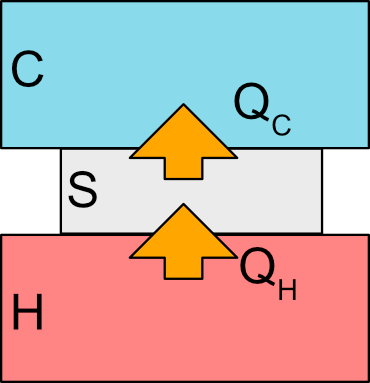
\includegraphics[width=6cm]{system} \caption{System (S) model}
\label{Fig2} 
\end{figure}

Treating the heater and the cooler as the environment, we can think of our system $S$ as an open system.
Further on we'll analyze the system $S$ from the perspective of internal $(i)$ entropy production
and external $(e)$ entropy flux, flowing \emph{to} the system $S$. 
Of course the change in entropy will be the sum of those two contributions:
\begin{equation}
dS_S=dS_i+dS_e.
\label{entrosum}
\end{equation}

In the current analysis let's consider a situation in which the same amount of heat flows in as flows out, that is $dQ_C=-dQ_H$. Using this relation we get the following term for the change of entropy:
\begin{equation}
dS_e=\frac{dQ_H}{T_H}+\frac{dQ_C}{T_C}=dQ_H\left(\frac{1}{T_H}-\frac{1}{T_C}\right)
=dQ_H\left(\frac{T_C-T_H}{T_HT_C}\right)<0.
\label{dSe1}
\end{equation}
From which it follows, that the heat flow takes the entropy out of our system.
For the purpose of further discussion we introduce the concept of rate of entropy change connected with the heat flow:
\begin{equation}
j_e \equiv  \frac{dS_e}{dt}. 
\end{equation}
In the considered scenerio, the $j_e$ is held constant (steady-state) and we suspect a continuous fall in system's entropy

Yet, moving away from the equilibrium state we suspect, that the a major role will be played by $dS_i$ moving the system back to equilibrium state. Similarly, as before we define the rate of internal entropy production:

\begin{equation}
j_i \equiv \frac{dS_i}{dt}.   
\end{equation} 

When $T_H=T_C$, i.e. the system is in equilibrium with constant entropy $S_{EQ}$ then it follows that $j_i=0$.
Therefore the rate of internal entropy production $j_i$ should be a function  of system's entropy $S_S$, i.e. $j_i = j_i(S_S)$ with the boundary condition $j_i(S_S=S_{EQ})=0$. 

Near the equilibrium state $S_S=S_{EQ}$, we can Taylor expand the function $j_i(S_S)$ to it's linear term
\begin{equation}
j_i(S_S)=j_i\left(S_{EQ}\right)+\left(S_S-S_{EQ}\right)C_1+\mathcal{O}\left(S_S^2\right),
\end{equation} 
fulfilling $j_i\left(S_{EQ}\right)=0$. 

The dimensional and stability analysis tells us that $C_1$ has the dimension of inverse time and in the case of 
$j_e=0$ should simply be equal to $S_{EQ}$, therefore we set $C_1 = -\frac{1}{\tau}$, where $\tau$ is a positive defined relaxation constant.

Using the equation (\ref{entrosum}) we get
\begin{equation}
\frac{dS_S}{dt}=j_i\left(S_S\right)=\left(S_S-S_{EQ}\right)C_1, 
\label{stab}
\end{equation} 

The solution of the equation (\ref{stab}) is then
\begin{equation}
S_S(t) =S_{EQ}+(S_0-S_{EQ})e^{-t/\tau}, 
\end{equation}
where the initial condition was set $S_S(0)=S_0$.


Now we include the term $j_e$ into our considerations.
In this case the equation (\ref{entrosum}) results in the following 
\begin{equation}
\frac{dS_S}{dt}=j_e + j_i\left(S_S\right)=j_e +\frac{S_{EQ}-S_S}{\tau}.
\label{dSSdt}
\end{equation} 

 
Given a boundary condition $S_S(0) =S_{EQ}$ it has a solution
\begin{equation}
S_S(t)=S_{EQ}+j_e\tau \left(1-e^{-t/\tau }\right),
\end{equation} 
where $j_e$ is a negative constant (graph of this function is presented on \ref{Fig4}). 
In the limit $t\rightarrow \infty$ the entropy of the system falls to the minimal value
\begin{equation}
S_{min}=S(t\rightarrow \infty) =S_{EQ}+j_e \tau < S_{EQ}.
\end{equation}

\begin{figure}[ht!]
\centering 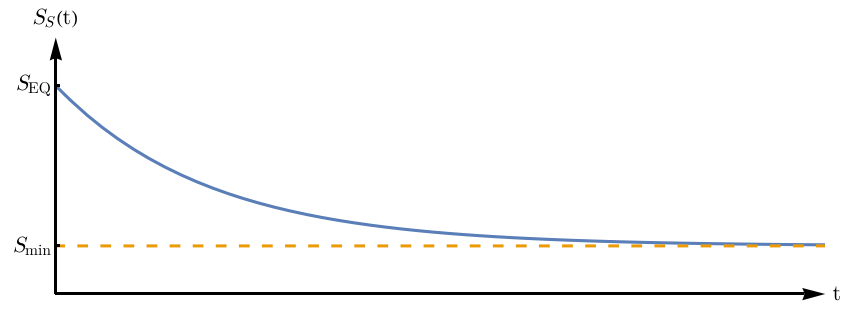
\includegraphics[width=12cm]{wykres3} 
\caption{Inducing lower entropy with heat flow.}
\label{Fig4} 
\end{figure}

This is of course consistent with the second law of thermodynamics as we're describing an open system.
It's easy to notice that the total entropy change is equal to $dS=dS_i \geq 0$ (for simplicity it was assumed that the heater and cooler don't act as producers of entropy).

\section{Pure non-equilibrium results}

In case of pure non-equilibrium fewer results are known in general.

In ordinary statistical physics when transitions between two equilibrium states are performed infinitely slowly along some path between the initial point $A$ and the final point $B$, then the total work $W$ performed on such a system is equal to the Helmholtz free energy difference $\Delta F$ between the initial and final configurations. However, this is not the case when non-equilibrium transitions are considered. In fact, on average the work performed on the system will exceed Helmholtz free energy $ \langle  W \rangle \geq \Delta F $ and the difference will be equal to the dissipated energy, associated with increase of entropy during an irreversible process.

\subsection{Jarzyński equality}

In 1996, Christopher Jarzynski\cite{Jarzynski:1997uj} derived a very useful equality for the equilibrium free energy differences between two configuration of a system in terms of an ensemble finite-time measurements of the work performed during parametric switching in between those two configurations.

\begin{equation}
\label{JarzynskiInequality}
  \langle \exp(-\beta W) \rangle = \exp(-\beta  \Delta F)
\end{equation}

\subsection{Crooks fluctuation theorem}

\subsection{Onsager-Machlup path integrals}


\subsection{Evans derivation}



\subsection{Appropriate treatment of reverse trajectories}

Let's consider a generic system statistical mechanical system a two times, an initial time $t_0$ and a final time $t_1$, each described by a complete set of possible macrostates $\{A_i\}$ for $ i=1,...,N_A $ and $\{B_j\}$ for $ j=1,...,N_B $  respectively. Each macrostate consists of some number of corresponding microstates denoted by $M_i$ for the initial macrostates and $N_j$ for the final macrostates. The deterministic, microscopic equations of motion then evolve a certain number of the microstates $K_{ij}$ from an initial macrostate $A_i$ to some final macrostate $B_j$.

The probability of the forward transition $P(B_j|A_i)$ is then equal to
\begin{equation}
  P(B_j|A_i)= \frac{K_{ij}}{M_i}
\end{equation}

Now for the time reversed case, that is to obtain $P(A_i|B_j)$, we use the Bayes theorem

\begin{equation}
  P(A_i|B_j)=\frac{P(B_j|A_i)P(A_i)}{P(B_j)},
\end{equation}

but on the way of doing so, we note that $A_i$ is still our "hypothesis" and $B_j$ is our evidence. Now, since we have no a priori knowledge about the initial macrostates, each of them is equally probable $P(A_i)= 1/N_A$.

$P(B_j)$ is then the marginal probability of evidence in all contradicting hypotheses or in other words a normalization factor obtained using the relation 

\begin{equation}
  \sum_i P(A_i|B_j) = 1
\end{equation}
which leads to $P(B_j) = \sum_i P(B_j|A_i)P(A_i)$. Using this we obtain the following expression for the post-diction

\begin{equation}
\begin{aligned}
  P(A_i|B_j) &= \frac{K_{ij}}{M_i} P(A_i) ( \sum_k \frac{K_{kj}}{M_k}P(A_k) )^{-1}\\
  &= \frac{K_{ij}}{M_i} ( \sum_{k,m} \frac{K_{kj}}{K_{km}})^{-1}
\end{aligned}
\end{equation}

where in the last equation we made use of the fact that $\sum_m K_{km}=M_k $.
This form is especially useful, because the matrix elements can be normalized and effectively we obtain a stochastic description.

It is important to emphasize that the conditional probabilities $P(B_j|A_i)$ and $P(A_i|B_j)$ are entirely different in nature - the first represents a prediction, but the second is a post-diction. There is no symmetry between assumptions and assertions in conditional probability calculus.

Using those results one may obtain the correct measure of irreversibility, comparing the probability of forward macroscopic evolution to backward probability evolution, called (but not derived) by Evans, dissipation function:

\begin{equation}
  \frac{P(B_j|A_i)}{P(A_i|B_j)}= e^{\ln{\sum_{k,m} \frac{K_{kj}}{K_{km}}}}
\end{equation}

Using random matrices, satisfying the conditions $\sum_j K_{kj} = 1$ for any $k$, one can obtain the distributions for the possible values of $ \Omega_t = \ln{\sum_{k,m} \frac{K_{kj}}{K_{km}}} $ presented on figure \ref{Fig4}.

\begin{figure}[ht!]
\centering 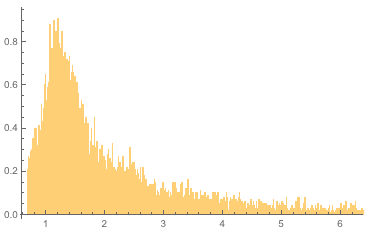
\includegraphics[width=8cm]{dissipation} \caption{Distribution of generic dissipation function for $N_A = 5$ and $N_B=3$}
\label{Fig4} 
\end{figure}

\newpage

\bibliographystyle{ieeetr}
\bibliography{Refs}


\end{document}